%%%%%%%%%%%%%%%%%%%%%%%%%%%%%%%%%%%%%%%%%%%%%%%%%%%%%%%%%%%%%%%%%%%%%%%%%%
% Signal of uT1 for lowing load
%%%%%%%%%%%%%%%%%%%%%%%%%%%%%%%%%%%%%%%%%%%%%%%%%%%%%%%%%%%%%%%%%%%%%%%%%%
\begin{solutionfigure}[htb]

 %   \documentclass{standalone}
 %   \usepackage{pgfplots}
 %   \pgfplotsset{compat=1.18} % Kompatibilität für neuere Versionen
        \centering
        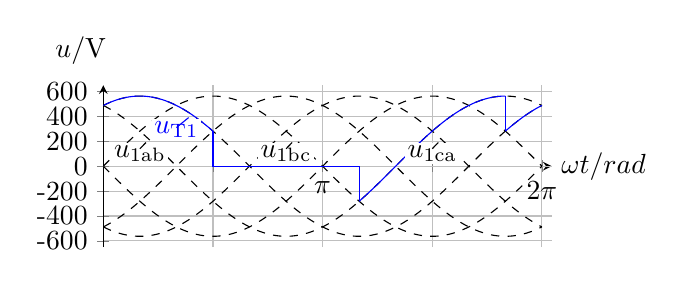
\begin{tikzpicture}
            \begin{axis}[
                % x/y range adjustment
                xmin=0, xmax=368,
                ymin=-650, ymax=650,
                samples=500,
                axis y line=center,
                axis x line=middle,
                extra y ticks=0,
                % Label text
                xlabel={$\omega t / \text{rad}$},,
                ylabel={$u/\mathrm{V}$},
                % Label adjustment
                x label style={at={(axis description cs:1,0.5)},anchor=west},
                y label style={at={(axis description cs:-.05,.97)},anchor=south,yshift=0.2cm},
                width=0.6\textwidth,
                height=0.3\textwidth,
                % x-Ticks
                xtick={0,90,180,270,360},
                xticklabels={,,$\pi$,,$2\pi$},
                xticklabel style = {anchor=north},
                % y-Ticks
                ytick={600,400,200,0,-200,-400,-600},
                yticklabels={600,400,200,0,-200,-400,-600},
                yticklabel style = {anchor=east},
                % Grid layout
                grid,
                %grid style={line width=.1pt, draw=gray!10},
                %major grid style={line width=.2pt,draw=gray!90},
            ]
            % Voltage u1ab(wt), u1bc(wt) u1ca(wt)
            \addplot[black, domain= 0:360,dashed] {563*cos(x-30)};                
            \addplot[black, domain= 0:360,dashed] {563*cos(x+210)}; 
            \addplot[black, domain= 0:360,dashed] {563*cos(x+90)};   
            % Voltage -u1ab(wt), -u1bc(wt) -u1ca(wt)
            \addplot[black, domain= 0:360,dashed] {-563*cos(x-30)};                
            \addplot[black, domain= 0:360,dashed] {-563*cos(x+210)}; 
            \addplot[black, domain= 0:360,dashed] {-563*cos(x+90)};
            % Voltage uT1(wt)
            \addplot[blue, domain= 0:90] {563*cos(x-30)};                
            \addplot[blue, domain= 210:330] {-563*cos(x+210)};             
            \addplot[blue, domain= 330:360] {563*cos(x-30)};             
            \addplot[color=blue,solid] coordinates{
                (90, 282)
                (90, 0)
                (210, 0)
                (210, -282)
            };     
            \addplot[color=blue,solid] coordinates{
                (330, 563)
                (330, 282)
            };     
            % Label of u1ab
            \node[black, fill=white, inner sep = 1pt, anchor = south] at (axis cs:30,10) {$u_{\mathrm{1ab}}$};
            % Line to +u1ab
            \draw[thin, black] (30,140) -- (35,190);            
            % Label of u1bc
            \node[black, fill=white, inner sep = 1pt, anchor = south] at (axis cs:150,10) {$u_{\mathrm{1bc}}$};
            % Line to +u1bc
            \draw[thin, black] (150,140) -- (155,190);            
            % Label of u1ca
            \node[black, fill=white, inner sep = 1pt, anchor = south] at (axis cs:270,10) {$u_{\mathrm{1ca}}$};
            % Line to +u1ca
            \draw[thin, black] (270,140) -- (275,190);            
            % Label of uT1
            \node[blue, fill=white, inner sep = 1pt, anchor = south] at (axis cs:60,200) {$u_{\mathrm{T1}}$};
            % Line to uT1
            \draw[thin, blue] (60,310) -- (70,390);
        \end{axis}     
        \end{tikzpicture}
        \caption{Voltage $u_\mathrm{T1}(\omega t)$ for lowering the load.}
        \label{sfig:ex06_Voltage_u1T_down}
\end{solutionfigure}